\chapter{AMOVA and Statistical phylogeography}

The notation now becomes just a little bit more complicated. We will
now use $x_{ik}$ to refer to the frequency of the $i$th haplotype in
the $k$th population. Then
\[
x_{i\cdot} = \frac{1}{K}\sum_{k=1}^K x_{ik}
\]
is the mean frequency of haplotype $i$ across all populations, where
$K$ is the number of populations. We can now define
\begin{eqnarray*}
\pi_t &=& \sum_{ij} x_{i\cdot}x_{j\cdot} \delta_{ij} \\
\pi_s &=& \frac{1}{K}\sum_{k=1}^K\sum_{ij} x_{ik}x_{jk}\delta_{ij} \quad ,
\end{eqnarray*}
where $\pi_t$ is the nucleotide sequence diversity across the entire
set of populations and $\pi_s$ is the average nucleotide sequence
diversity within populations. Then we can define\index{nucleotide diversity!partitioning}
\begin{equation}
\Phi_{st} = \frac{\pi_t - \pi_s}{\pi_t} \quad ,
\label{eq:phi-st}
\end{equation}
which is the direct analog of Wright's $F_{st}$ for nucleotide
sequence diversity. Why? Well, that requires you to remember stuff we
covered eight or ten weeks ago.\index{Phi-st@$\Phi_{st}$}\index{AMOVA}

To be a bit more specific, refer back to
\url{http://darwin.eeb.uconn.edu/eeb348/lecture-notes/wahlund/node4.html}.
If you do, you'll see that we defined
\[
F_{IT} = 1 - \frac{H_i}{H_t} \quad ,
\]
where $H_i$ is the average heterozygosity in individuals and $H_t$ is
the expected panmictic heterozygosity. Defining $H_s$ as the average
panmictic heterozygosity within populations, we then observed that
\begin{eqnarray*}
1 - F_{IT} &=& \frac{H_i}{H_t} \\
           &=& \frac{H_i}{H_s}\frac{H_s}{H_t} \\
           &=& (1 - F_{IS})(1 - F_{ST}) \\
1-F_{ST} &=& \frac{1-F_{IT}}{1-F_{IS}} \\
F_{ST} &=&
\frac{\left(1-F_{IS}\right)-\left(1-F_{IT}\right)}{1-F_{IS}} \\
&=& \frac{\left(H_i/H_s\right) - \left(H_i/H_t\right)}{H_i/H_s} \\
&=& 1 - \frac{H_s}{H_t} \quad .
\end{eqnarray*}
In short, another way to think about $F_{ST}$ is
\begin{equation}
F_{ST} = \frac{H_t - H_s}{H_t} \quad .
\label{eq:f-st}
\end{equation}
Now if you compare equation~(\ref{eq:phi-st}) and
equation~(\ref{eq:f-st}), you'll see the analogy.

So far I've motivated this approach by thinking about $\delta_{ij}$ as
the fraction of sites at which two haplotypes differ and $\pi_s$ and
$\pi_t$ as estimates of nucleotide diversity. But nothing in the
algebra leading to equation~(\ref{eq:phi-st}) requires that
assumption. Excoffier et al.~\cite{Excoffier-etal92} pointed out that
other types of molecular data can easily be fit into this
framework. We simply need an appropriate measure of the ``distance''
between different haplotypes or alleles. Even with nucleotide
sequences the appropriate $\delta_{ij}$ may reflect something about
the mutational pathway likely to connect sequences rather than the raw
number of differences between them. For example, the distance might be
a Jukes-Cantor distance or a more general distance measure that
accounts for more of the properties we know are associated with
nucleotide substitution. The idea is illustrated in
Figure~\ref{fig:amova-procedure}. Once we have $\delta_{ij}$ for all
pairs of haplotypes or alleles in our sample, we can use the ideas
lying behind equation~(\ref{eq:phi-st}) to partition
diversity{\dash}the average distance between randomly chosen
haplotypes or alleles{\dash}into within and among population
components.\footnote{As with $F$-statistics, the actual estimation
  procedure is more complicated than I describe here. Standard
  approaches to AMOVA use method of moments calculations analogous to
  those introduced by Weir and Cockerham for
  $F$-statistics~\cite{WeirCockerham84}. Bayesian approaches are
  possible, but they are not yet widely available~(meaning, in part,
  that I know how to do it, but I haven't written the necessary
  software yet).} This procedure for
partitioning diversity in molecular markers is referred to as an
analysis of molecular variance or AMOVA (by analogy with the
ubiquitous statistical procedure analysis of variance, ANOVA). Like
Wright's $F$-statistics, the analysis can include several levels in
the hierarchy.

\begin{figure}
\begin{center}
\resizebox{!}{8cm}{\includegraphics{amova-procedure.eps}}
\end{center}
\caption{Converting raw differences in sequence (or presence and
  absence of restriction sites) into a minimum spanning tree and a
  mutational measure of distance for an analysis of molecular variance~(from~\cite{Excoffier-etal92}).}\label{fig:amova-procedure}
\end{figure}

\section*{An AMOVA example}\index{AMOVA!example}

Excoffier et al.~\cite{Excoffier-etal92} illustrate the approach by
presenting an analysis of restriction haplotypes in human mtDNA. They
analyze a sample of 672 mitochondrial genomes representing two
populations in each of five regional
groups~(Figure~\ref{fig:amova-sample-locations}). They identified 56
haplotypes in that sample. A minimum spanning tree illustrating the
relationships and the relative frequency of each haplotype is
presented in Figure~\ref{fig:amova-haplotypes}.

\begin{figure}
\begin{center}
\resizebox{!}{6cm}{\includegraphics{amova-sample-locations.eps}}
\end{center}
\caption{Locations of human mtDNA samples used in the example
  analysis~(from~\cite{Excoffier-etal92}).}\label{fig:amova-sample-locations}
\end{figure}

\begin{figure}
\begin{center}
\resizebox{!}{6cm}{\includegraphics{amova-haplotypes.eps}}
\end{center}
\caption{Minimum spanning network of human mtDNA samples in the
  example. The size of each circle is proportional to its
  frequency~(from~\cite{Excoffier-etal92}).}\label{fig:amova-haplotypes}
\end{figure}

It's apparent from the figure that haplotype 1 is very common. In
fact, it is present in substantial frequency in every sampled
population. An AMOVA using the minimum spanning network in
Figure~\ref{fig:amova-haplotypes} to measure distance produces the
results shown in Table~\ref{table:amova-results}. Notice that there is
relatively little differentiation among populations within the same
geographical region ($\Phi_{SC} = 0.044$). There is, however,
substantial differentiation among regions ($\Phi_{CT} = 0.220$). In
fact, differences among populations in different regions is
responsible for nearly all of the differences among populations
($\Phi_{ST} = 0.246$). Notice also that $\Phi$-statistics follow the
same rules as Wright's $F$-statistics, namely
\begin{eqnarray*}
1 - \Phi_{ST} &=& (1 - \Phi_{SC})(1 - \Phi_{CT}) \\
0.754 &=& (0.956)(0.78) \quad ,
\end{eqnarray*}
within the bounds of rounding error.\footnote{There wouldn't be any
  rounding error if we had access to the raw data.}

\begin{table}
\begin{center}
\begin{tabular}{lc}
\hline\hline
Component of differentiation     & $\Phi$-statistics \\
\hline
Among regions                    & $\Phi_{CT} = 0.220$ \\
Among populations within regions & $\Phi_{SC} = 0.044$ \\
Among all populations            & $\Phi_{ST} = 0.246$ \\
\hline
\end{tabular}
\end{center}
\caption{AMOVA results for the human mtDNA
  sample~(from~\cite{Excoffier-etal92}).}\label{table:amova-results}
\end{table}

\section*{An extension}

As you may recall,\footnote{Look back at
  \url{http://darwin.eeb.uconn.edu/eeb348/lecture-notes/coalescent/node6.html}
  for the details.}
Slatkin~\cite{Slatkin91-coalescence} pointed out that there is a
relationship between coalescence time and $F_{st}$. Namely, if
mutation is rare then
\[
F_{ST} \approx \frac{\bar t - \bar t_0}{\bar t} \quad ,
\]
where $\bar t$ is the average time to coalescence for two genes drawn
at random without respect to population and $\bar t_0$ is the average
time to coalescence for two genes drawn at random from the same
populations. Results in~\cite{Holsinger-MasonGamer96} show that when
$\delta_{ij}$ is linearly proportional to the time since two sequences
have diverged, $\Phi_{ST}$ is a good estimator of $F_{ST}$ when
$F_{ST}$ is thought of as a measure of the relative excess of
coalescence time resulting from dividing a species into several
population. This observation suggests that the combination of
haplotype frequency differences and evolutionary distances among
haplotypes may provide insight into the evolutionary relationships
among populations of the same species.

\section*{Statistical phylogeography: a preview}

Nested clade analysis represented the earliest attempt to develop a
formal approach to using an estimate of phylogenetic relationships
among haplotypes to infer something both about the biogeographic
history of the populations in which they are contained and the
evolutionary processes associated with the pattern of diversification
implied by the phylogenetic relationships among haplotypes and their
geographic distribution. The statistical parsimony part of NCA depends
heavily on coalescent theory for calculating the ``limits'' of
parsimony. As a result, NCA combines aspects of pure phylogenetic
inference{\dash}parsimony{\dash}with aspects of pure population
genetics{\dash}coalescent theory{\dash}to develop a set of inferences
about the phylogeographic history of populations within species. But
well before NCA was developed, Pamilo and Nei~\cite{Pamilo-Nei-1988}
pointed out that the phylogenetic relationships of a single gene might
be different from those of the populations from which the samples were
collected.

\section*{Gene trees {\it versus\/} population trees}\index{gene tree}\index{population tree}

There are several reasons why {\it gene trees\/} might not match {\it
  population trees}.

\begin{itemize}

\item It could simply be a problem of estimation. Given a particular
  set of gene sequences, we {\it estimate} a phylogenetic relationship
  among them. But our estimate could be wrong. In fact, given the
  astronomical number of different trees possible with 50 or 60
  distinct sequences, it's virtually certain to be wrong somewhere. We
  just don't know where. It could be that if we had the right gene
  tree it would match the species tree.

\item There might have been a hybridization event in the past so that
  the phylogenetic history of the gene we're studying is different
  from that of the populations from which we sampled. Hybridization is
  especially likely to have a large impact if the locus for which we
  have information is uniparentally inherited, e.g., mitochondrial or
  chloroplast DNA. A single hybridization event in the distant past in
  which the maternal parent was from a different population will give
  mtDNA or cpDNA a very different phylogeny than nuclear genes that
  underwent a lot of backcrossing after the hybridization event.

\item If the ancestral population was polymorphic at the time the
  initial split occurred alleles that are more distantly related
  might, by chance, end up in the same descendant population~(see
  Figure~\ref{fig:ancestral-polymorphism})\index{ancestral polymorphism}

\end{itemize}

\begin{figure}
\begin{center}
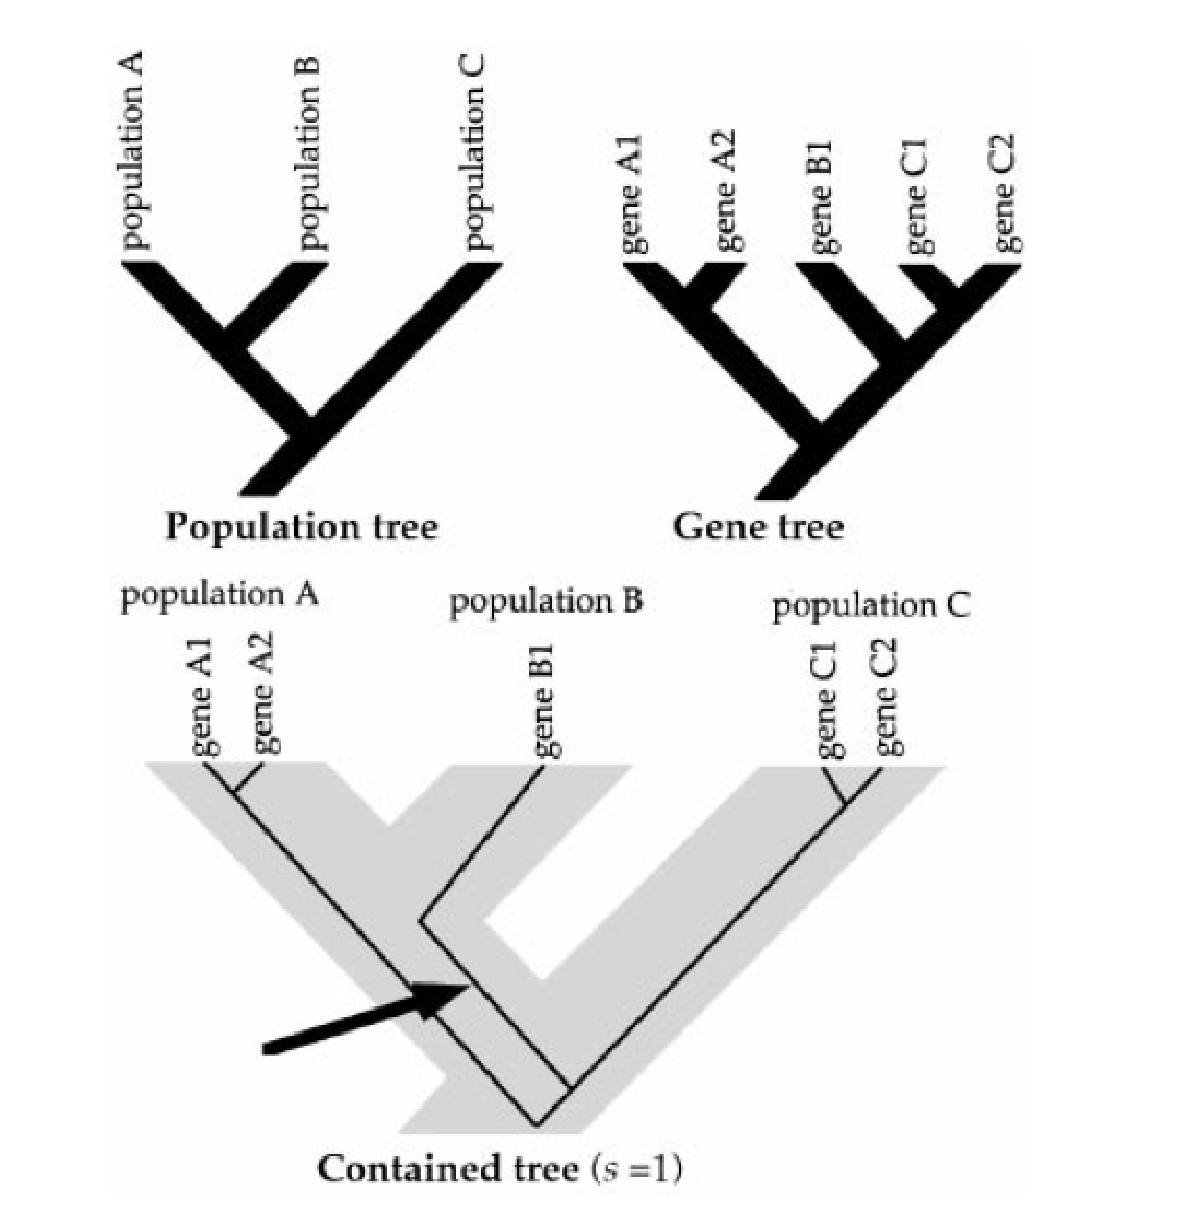
\includegraphics[height=6cm]{ancestral-polymorphism.eps}
\end{center}
\caption{Discordance between gene and population trees as a result of
  ancestral polymorphism
  (from~\cite{Knowles-2001}).}\label{fig:ancestral-polymorphism} 
\end{figure}

As Pamilo and Nei showed, it's possible to calculate the probability
of discordance between the gene tree and the population tree using
some basic ideas from coalescent theory. That leads to a further
refinement, using coalescent theory directly to examine alternative
biogeographic hypotheses.

\section*{Phylogeography of montane grasshoppers}

Lacey Knowles studied grasshoppers in the genus {\it Melanopus}. She
collected 1275bp of DNA sequence data from cytochrome oxidase I (COI)
from 124 individuals of {\it M. oregonensis\/} and two outgroup
speices. The specimens were collected from 15 ``sky-island'' sites in
the northern Rocky Mountains~(see Figure~\ref{fig:sky-islands};
\cite{Knowles-2001}). Two alternative hypotheses had been proposed to
describe the evolutionary relationships among these
grasshoppers~(refer to Figure~\ref{fig:divergence-hypotheses} for a
pictorial representation):\index{Melanopus@\textit{Melanopus}}

\begin{figure}
\begin{center}
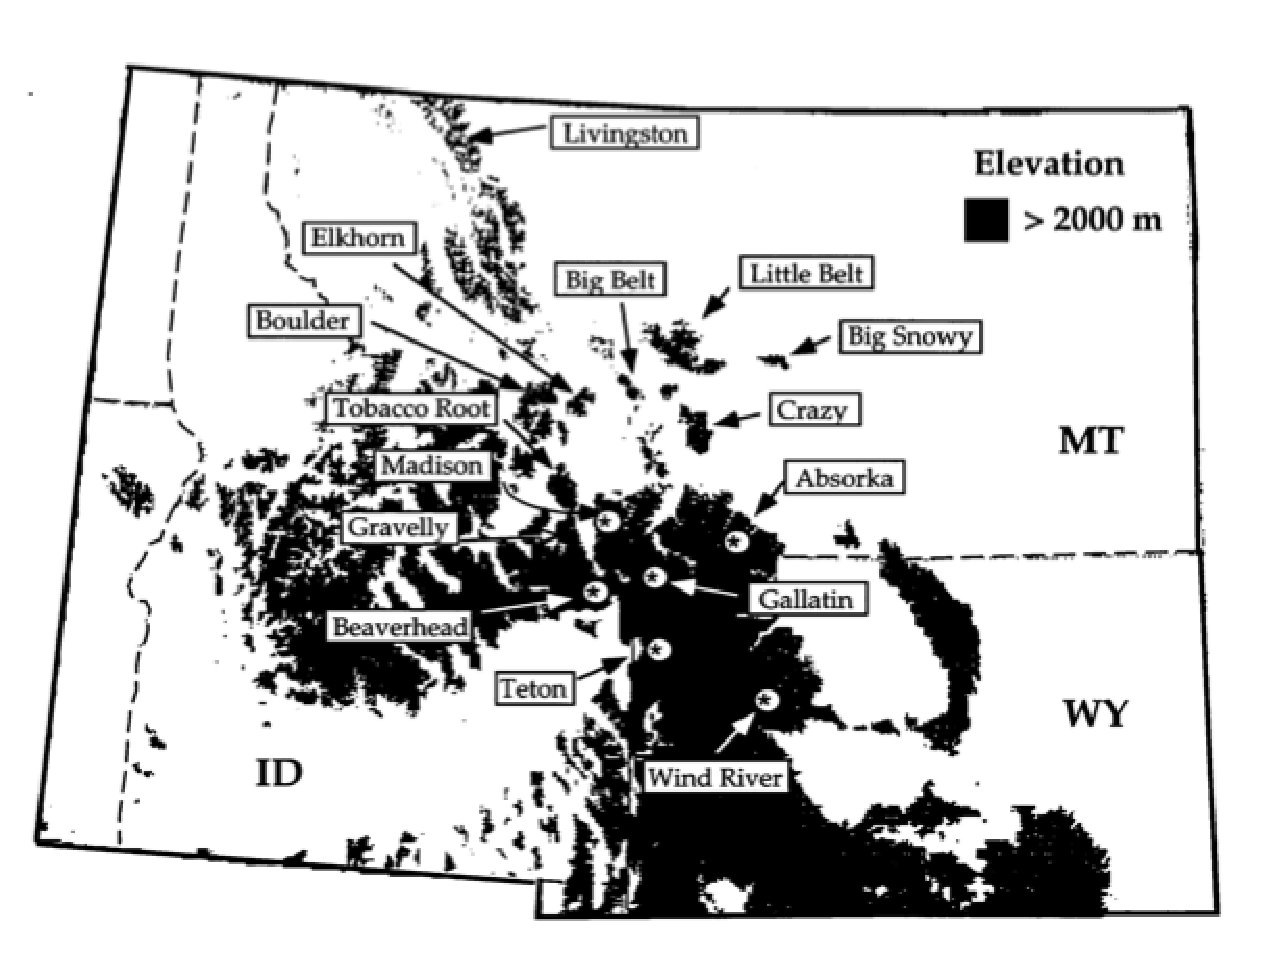
\includegraphics[height=6cm]{sky-islands.eps}
\end{center}
\caption{Collection sites for {\it Melanopus oregonensis\/} in the
  northern Rocky Mountains~(from~\cite{Knowles-2001}).}\label{fig:sky-islands}
\end{figure}

\begin{itemize}

\item {\bf Widespread ancestor}: The existing populations might represent
  independently derived remnants of a single, widespread
  population. In this case all of the populations would be equally
  related to one another.

\item {\bf Multiple glacial refugia}: Populations that shared the same
  refugium will be closely related while those that were in different
  refugia will be distantly related.

\end{itemize}

\begin{figure}
\begin{center}
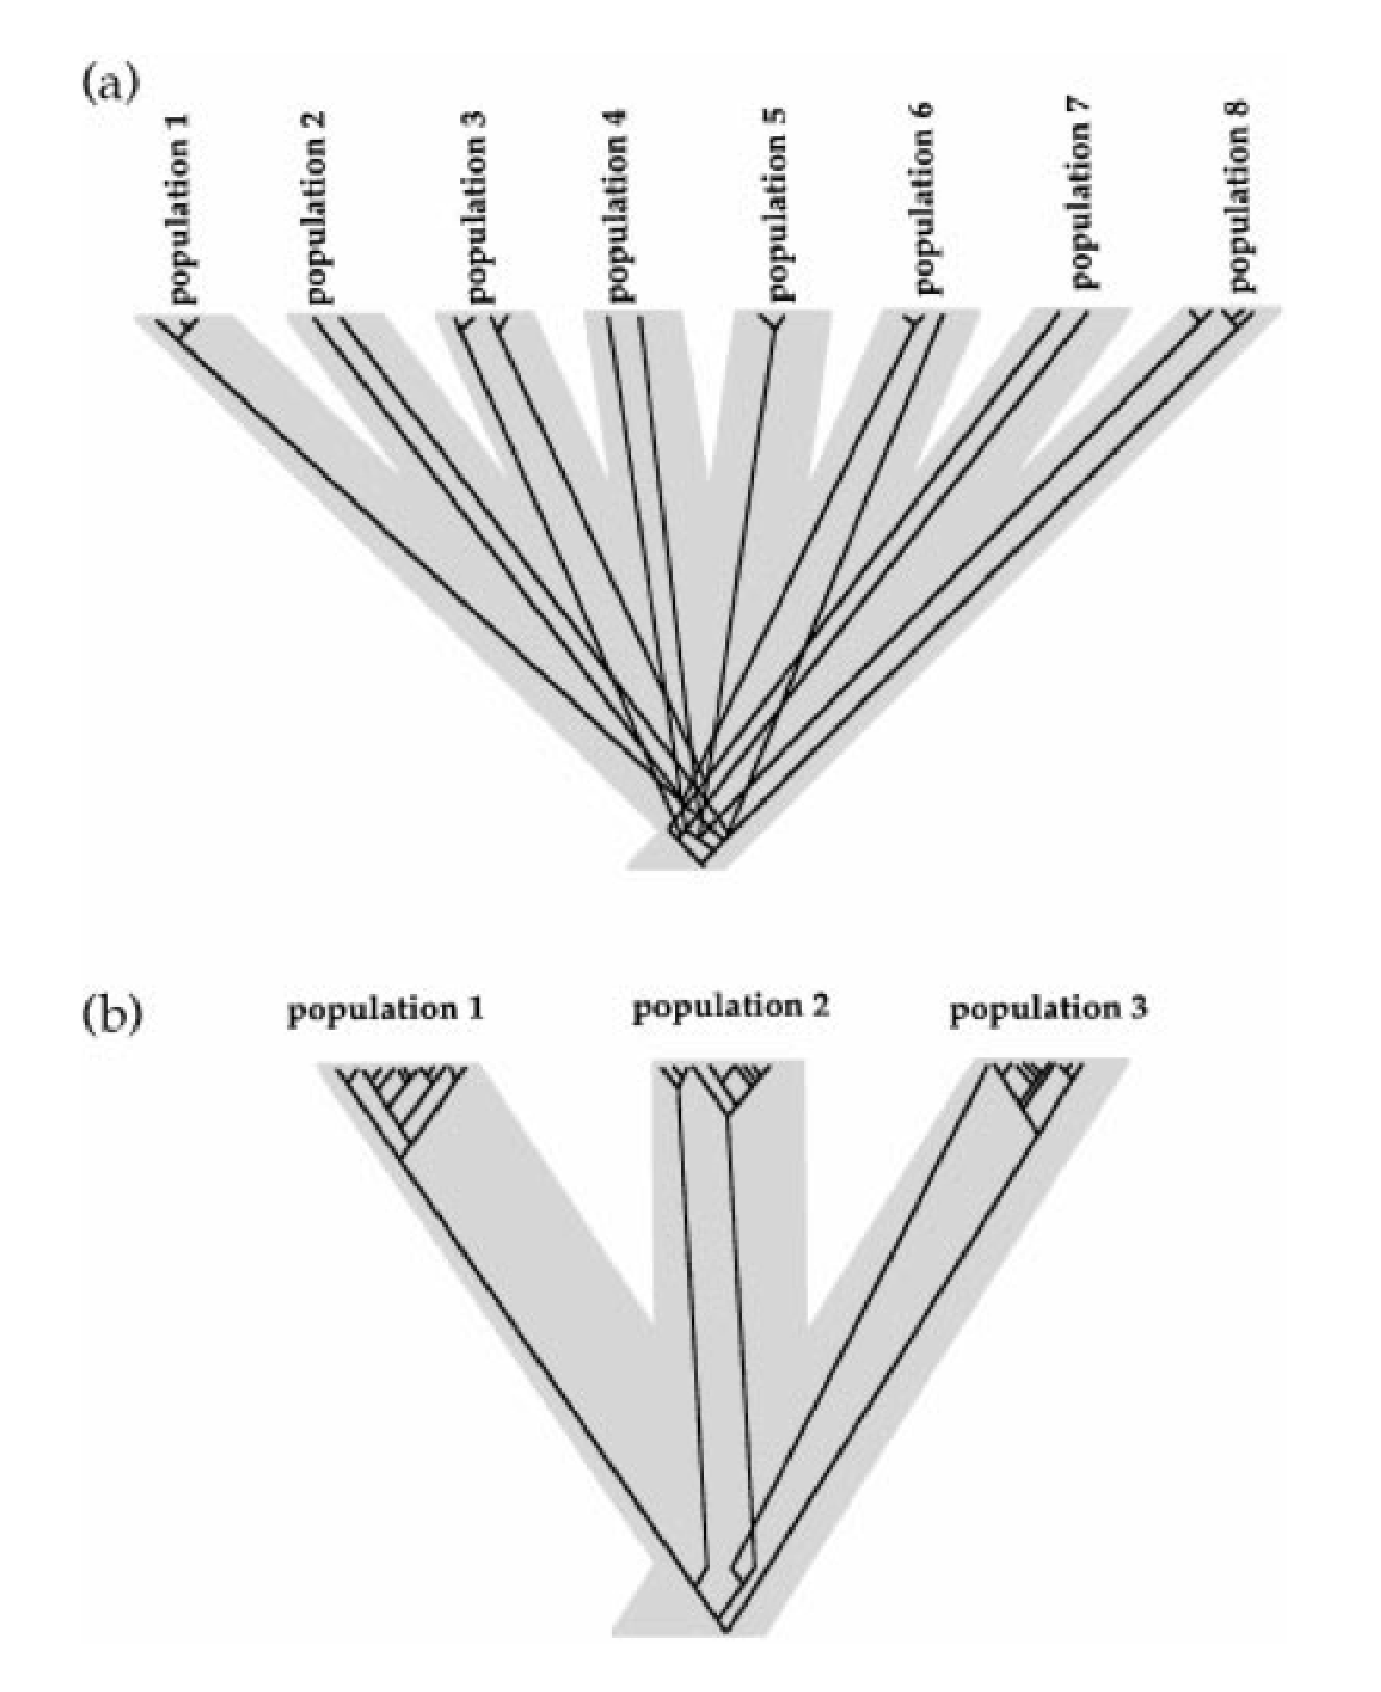
\includegraphics[height=6cm]{divergence-hypotheses.eps}
\end{center}
\caption{Pictorial representations of the ``widespread ancestor''
  (top) and ``glacial refugia'' (bottom)
  hypotheses~(from~\cite{Knowles-2001}).}\label{fig:divergence-hypotheses}
\end{figure}

As is evident from Figure~\ref{fig:divergence-hypotheses}, the two
hypotheses have very different consequences for the coalescent history
of alleles in the sample. Since the interrelationships between
divergence times and time to common ancestry differ so markedly
between the two scenarios, the pattern of sequence differences found
in relation to the geographic distribution will differ greatly between
the two scenarios. 

Using techniques described in Knowles and
Maddison~\cite{Knowles-Maddison-2002}, Knowles simulated gene trees
under the widespread ancestor hypothesis. She then placed them within
a population tree representing the multiple glacial refugia hypothesis
and calculated a statistic, $s$, that measures the discordance between
a gene tree and the population tree that contains it. This gave her a
distribution of $s$ under the widespread ancestor hypothesis. She
compared the $s$ estimated from her actual data with this distribution
and found that the observed value of $s$ was only 1/2 to 1/3 the size
of the value observed in her simulations.\footnote{The discrepancy was
  largest when divergence from the widespread ancestor was assumed to
  be very recent.} In short, Knowles presented strong evidence that
her data are not consistent with the widespread ancestor
hypothesis.\index{statistical phylogeography!example}

